\documentclass[12pt]{standalone}

\usepackage{tikz}

\usetikzlibrary{angles,quotes,arrows.meta}

\begin{document}
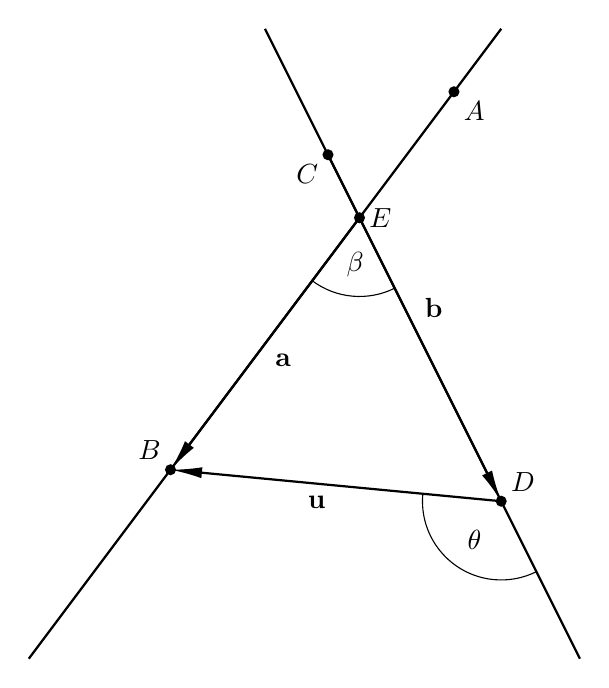
\begin{tikzpicture}[angle radius=1cm]

\begin{scope}[thick]
    \draw (2,4) coordinate (M)
        -- coordinate[pos=0.1] (A)
        coordinate[pos=0.7] (B)
        (-4,-4) coordinate (N);
    \draw (-1,4) coordinate (P)
        -- coordinate[pos=0.2] (C)
        coordinate[pos=0.75] (D)
        (3,-4) coordinate (Q);
\end{scope}

\coordinate (E) at (intersection cs:first line={(A)--(B)},
    second line={(C)--(D)});

\path[thick,-{Latex[width=4pt,length=4mm]}]
    (E) edge["$\bf a$"] (B)
    (C) edge["$\bf b$"] (D)
    (D) edge["$\bf u$"] (B);

\draw
    pic["$\beta$",draw=black] {angle = B--E--D}
    pic["$\theta$",draw=black] {angle = B--D--Q};

\fill (A) circle (2pt);
\fill (B) circle (2pt);
\fill (C) circle (2pt);
\fill (D) circle (2pt);
\fill (E) circle (2pt);

\node[below right] at (A) {$A$};
\node[above left] at (B) {$B$};
\node[below left] at (C) {$C$};
\node[above right] at (D) {$D$};
\node[right] at (E) {$E$};

\end{tikzpicture}
\end{document}
